\section{Concept E: Kinetic Bolas}  
Concept E uses a lift-and-cruise UAV to fire a kinetic bolas at the
balloon suspension line or lower flight train. The weighted projectiles
wrap around the line and create a high-friction anchor, after which the
UAV tows the balloon-payload system toward the recovery zone. During the
initial design phase, this option was compared with a payload-hover
drone and a collaborative tether concept. The power and battery-mass
comparison in \autoref{tab:drone_power_analysis} retained the kinetic
bolas option because the alternative tethered concepts required
excessive battery mass or operational complexity.

\begin{table}[H]
\centering
\caption{Comparative Analysis of Power Requirements and Battery Mass}
\label{tab:drone_power_analysis}
\begin{tabular}{lrrrrr}
\toprule
\textbf{Flight Metric} & \textbf{Bolas Quad} & \textbf{Bolas VTOL} & \textbf{Hover Quad} & \textbf{Hover VTOL} & \textbf{Tethered Drone} \\
\midrule
Hover Power (W)    & 2,881.65  & 4,075.26  & 6,830.57  & 9,659.88  & 23,053.17 \\
Climb Power (W)    & 7,296.15  & 5,699.14  & 15,659.57 & 5,794.75  & 40,711.17 \\
Cruise Power (W)  & 7,139.93  & 2,358.03  & 7,449.28  & 2,652.78  & 23,671.88 \\
Descent Power (W) & 17,842.01 & 17,842.01 & 18,350.96 & 19,781.72 & 23,053.17 \\
\midrule
Total Energy (kJ)  & 25,584    & 22,115    & 32,430    & 25,770    & 66,294    \\
Battery Mass (kg) & 40.38     & 34.90     & 51.18     & 40.67     & 104.63    \\
\bottomrule
\end{tabular}
\end{table}

\subsection{System Architecture}
\label{subsec:concept_E_architecture}
The Concept E architecture is represented by the conceptual impression
and bolas reference in \autoref{fig:combined_comparison}.

\begin{figure}[H]
     \centering
     \begin{subfigure}[b]{0.48\textwidth}
         \centering
         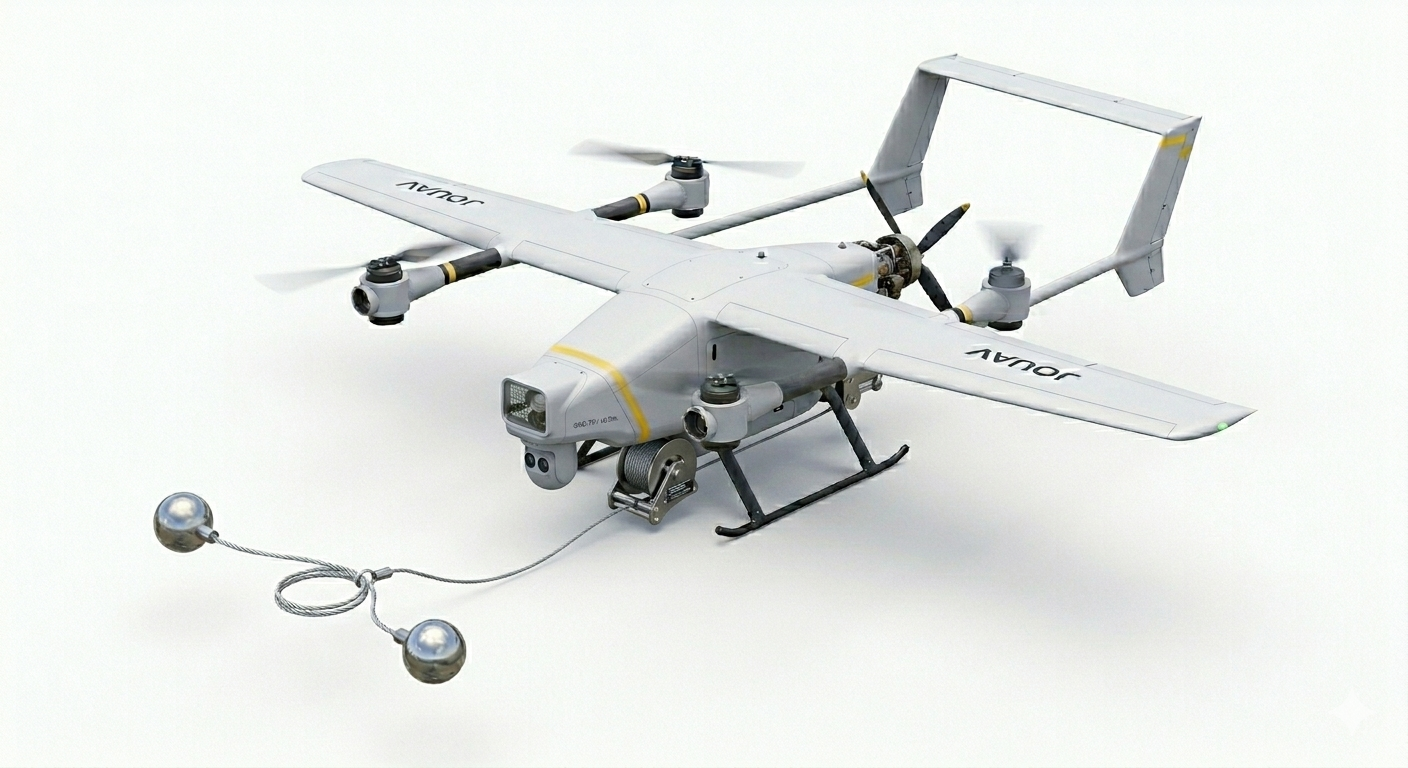
\includegraphics[width=\textwidth]{figures/Gemini_Generated_Image_9h0fwa9h0fwa9h0f.png}
         \caption{Initial impression}
         \label{fig:concept_e_ai}
     \end{subfigure}
     \hfill
     \begin{subfigure}[b]{0.25\textwidth}
         \centering
         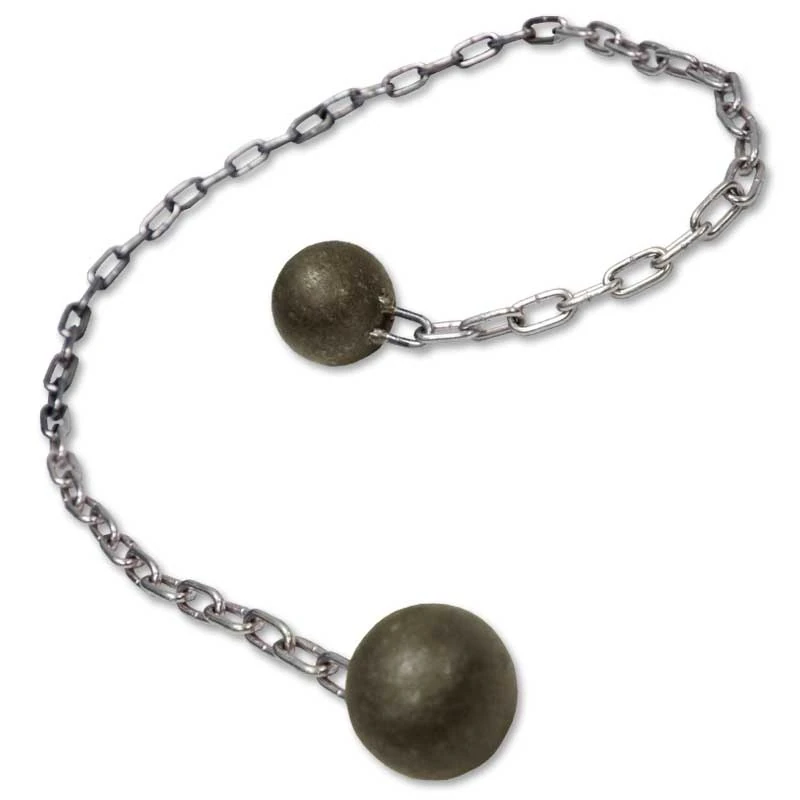
\includegraphics[width=\textwidth]{figures/Concepts/Bolas.png}
         \caption{Bolas reference example}
         \label{fig:bolas_reference}
     \end{subfigure}
     \caption{Concept E visual comparison. Left: author-generated concept impression; right: bolas reference example.}
     \label{fig:combined_comparison}
\end{figure}

\subsubsection{Aerial Platform}
A lift-and-cruise hybrid configuration is selected for efficient transit
and stable hover during launcher aiming. The firing phase requires
sub-metre lateral positioning next to the suspension line, so the
tail-sitter control risk during precision hover was treated as a
disadvantage for this concept. The lift-and-cruise layout also allows a
single forward sensor suite to support both transit and terminal
engagement.

\subsubsection{Sensing and Tracking}
Concept E uses the common external-cueing and terminal-sensing approach
from Section~\ref{sec:common_mission_assumptions}. Its concept-specific
sensing challenge is stable hover next to the suspension line during
bolas deployment, with a target relative-position error below
\(0.5~\mathrm{m}\). A nose-mounted sensor suite is used for preliminary
sizing, supported by tether-tension sensing to avoid overstressing the
suspension lines after engagement.

\subsubsection{Balloon Interaction Mechanism}
The UAS uses a pneumatic launcher to fire a bola: two weighted
projectiles connected by a high-strength leader line. The weights are
discharged from the engine pods with more than \(1~\mathrm{m}\) of
separation to increase the chance of wrapping around the vertical
suspension line. After contact, projectile momentum wraps the leader
around the line. The capstan effect increases friction with each wrap
and creates an anchor without a mechanical clamp. The UAS monitors
attachment through tension sensors; if the attachment is weak, it can
orbit the line to increase the wrap count. Ground support must reload
the expendable projectiles and inspect the launcher between missions.

\subsubsection{Descent Initiation}
After the bolas has wrapped around the vertical line, the UAS reels out
its tow line and applies a controlled downward and lateral load. The
vehicle uses its mass and directed thrust to overcome residual free lift
and start a managed descent.

\subsubsection{Descent Management and Recovery}
During descent, the UAS remains connected through the tow line and uses
directed thrust to steer the balloon-payload system toward the recovery
zone. The tethered configuration reduces continuous vertical thrust
demand, but it introduces pendulum dynamics, line-load limits, and
propeller-entanglement risk near the aircraft.

\subsection{Mass, Cost, and Power Estimates}
The initial mass estimate incorporates mass fractions, margins, and the allocation for the pneumatic bolas launcher, as shown in \autoref{tab:mass_fractions_bolas}.

\begin{table}[htbp]
\centering
\caption{Mass Fractions and Component Weights}
\label{tab:mass_fractions_bolas}
\begin{tabular}{lcccc}
\toprule
\textbf{Parameter} & Structure Fraction & Propulsion Fraction & Avionics Fraction & Launcher Weight (kg) \\
\midrule
\textbf{Value} & 0.27 & 0.27 & 0.05 & 3.75 \\
\bottomrule
\end{tabular}
\end{table}

Using the power-based mass iteration described in \autoref{sec:power_mass}, the power requirements and final mass distribution for the Lift+Cruise architecture were determined. These results are summarized in \autoref{tab:lift_cruise_power} and \autoref{tab:lift_cruise_weight}.

\begin{table}[H]
    \centering
    \begin{minipage}{0.48\textwidth}
        \centering
        \caption{Power and Energy Requirements}
        \label{tab:lift_cruise_power}
        \small
        \begin{tabular}{lr}
            \toprule
            \textbf{Parameter} & \textbf{Value} \\
            \midrule
            Hover power (W)    & 3,490.79 \\
            Cruise power (W)   & 754.22   \\
            Climb power (W)    & 5,174.05 \\
            Descent power (W)  & 4,000.00 \\
            \midrule
            Total energy (J)   & 7,004,195.17 \\
            Battery mass (kg)  & 11.05    \\
            \bottomrule
        \end{tabular}
    \end{minipage}
    \hfill 
    \begin{minipage}{0.48\textwidth}
        \centering
        \caption{Mass Breakdown}
        \label{tab:lift_cruise_weight}
        \small
        \begin{tabular}{lr}
            \toprule
            \textbf{Component} & \textbf{Mass [kg]} \\
            \midrule
            Structure \& frame  & 10.18 \\
            Propulsion          & 10.18 \\
            Avionics            & 1.88  \\
            Capture mechanism    & 3.75  \\
            Battery             & 11.05 \\
            Margin (10\%)       & 0.65  \\
            \midrule
            \textbf{ESTIMATED MTOW} & \textbf{37.69} \\
            \bottomrule
        \end{tabular}
    \end{minipage}
\end{table}

This initial estimate is corroborated by a review of off-the-shelf components, which also serves as the basis for cost estimation. A detailed breakdown is provided in \autoref{tab:component_breakdown}.


 
\small
\setlength{\LTleft}{0pt}
\setlength{\LTright}{0pt}
\setlength{\tabcolsep}{4pt}
\renewcommand{\arraystretch}{1.15}

\begin{longtable}{@{}
>{\raggedright\arraybackslash}p{0.30\textwidth}
r
r
>{\raggedright\arraybackslash}p{0.38\textwidth}
@{}}
\caption{Component Mass, Cost and Source Breakdown for Lift+Cruise UAS}
\label{tab:component_breakdown} \\
\toprule
\textbf{Component} & \textbf{Cost [EUR]} & \textbf{Mass [kg]} & \textbf{Source basis} \\
\midrule
\endfirsthead

\toprule
\textbf{Component} & \textbf{Cost [EUR]} & \textbf{Mass [kg]} & \textbf{Source basis} \\
\midrule
\endhead

\bottomrule
\endfoot

Battery system & 2,819.94 & 14.760 & \cite{TattuGmbH} \\
Lift motors & 1,519.60 & 3.960 & \cite{U13Drones} \\
Lift ESCs & 679.96 & 1.438 & \cite{ALPHAStability} \\
Lift propellers & 715.80 & 0.428 & \cite{G3211Store} \\
Cruise motor & 229.00 & 0.780 & \cite{AT7224Smooth} \\
Cruise ESC & 109.99 & 0.182 & \cite{T-MOTORController} \\
Cruise propeller & 118.90 & 0.080 & \cite{AUZPropeller} \\
Airframe structure & 2,000.00 & 7.900 & \cite{CarbonCompositesb,CarbonComposites,Aluminum7075-T651,CuredComposites} \\
Avionics suite & 973.97 & 0.659 & \cite{PixhawkStore,DroneCANStore,SiKStore,PM08-CANStore,AS150Amass,FLYRCGames,AlleDrones} \\
Bolas \& reel mechanism & 1,415.00 & 3.750 & \cite{GummiuberzogeneOse,D12Ltd,MarlowPB,UmarexPatronen,UmarexAccessoires,ASAZ-RAM.net,16mmComposites,RSRS,HS-5085MGRCD,CuredComposites} \\
Hardware \& wiring & 400.00 & 1.200 & \cite{AS150Amass,FLYRCGames,AlleDrones,CuredComposites} \\
\midrule
\textbf{Total} & \textbf{10,982.16} & \textbf{35.137} & -- \\

\end{longtable}
}
Additional sensing mass and cost margin should be confirmed during detailed sizing.
\subsubsection{Size Estimate}
The design leads to an initial weight estimate of approximately 37.3 kg. Sizing drivers include propeller diameter and wingspan. With a vertical propeller radius of 0.7 m, a horizontal propeller radius of 0.4 m, and a chord $c = 0.7$ m, the longitudinal extension is:
\begin{equation}
    L_x = 4 \cdot R_{VTOL} + 2 \cdot R_{FWD} = 2.4\,\text{m}
\end{equation}
Given a wing surface of 5.4 m$^2$, the resulting wingspan is 7.7 m. Consequently, the total footprint is $7.7\,\text{m} \times 2.5\,\text{m}$. 

\iffalse
\begin{figure}[H]
    \centering
    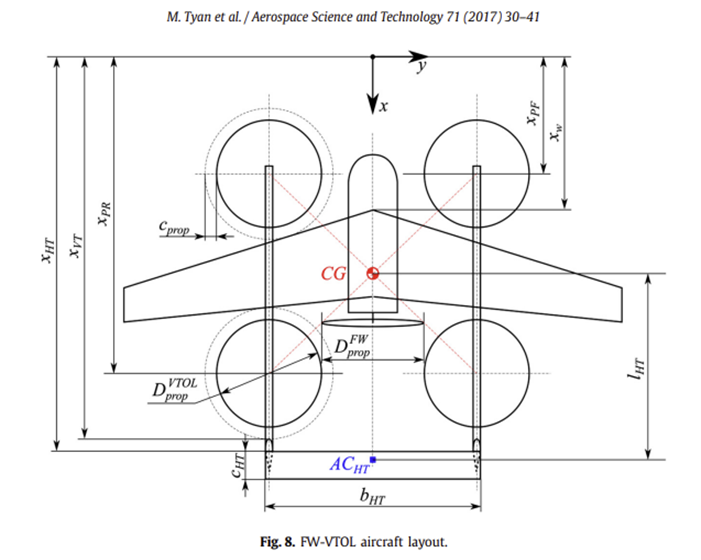
\includegraphics[width=0.7\linewidth]{figures/Concepts/lift_and_cruise.png}
    \caption{Lift-and-cruise UAS architecture selected for the recovery mission.}
    \label{fig:lift_and_cruise}
\end{figure}
\fi

\subsection{Risks and Uncertainties}
Operational risks for Concept E centre on ballistic accuracy,
line-wrapping reliability, and safe tow-line management after
attachment.

{
\small
\setlength{\LTleft}{0pt}
\setlength{\LTright}{0pt}

\begin{longtable}{p{0.27\textwidth} p{0.38\textwidth} p{0.30\textwidth}}
\caption{Key risks and mitigation strategies for the Kinetic Bolas concept.}
\label{tab:conceptE_key_risks} \\
\toprule
\textbf{Risk} & \textbf{Effect on mission} & \textbf{Possible mitigation} \\
\midrule
\endfirsthead

\toprule
\textbf{Risk} & \textbf{Effect on mission} & \textbf{Possible mitigation} \\
\midrule
\endhead

\bottomrule
\endfoot

Ballistic miss & The bolas misses or fails to wrap around the line. & Carry redundant projectiles and require a confirmed wrap before descent. \\
Line-wrap friction failure & Insufficient wrapping lets the bolas slide down the tether. & Use tension sensing and controlled orbiting manoeuvres to increase wrap count. \\
Tether overstress & Dynamic loads exceed the line safety factor (SF = 2.25). & Monitor line load and modulate thrust to reduce stress peaks. \\
Propeller entanglement & The tow line enters the rotor disk during transition or descent. & Maintain stand-off distance and consider protective shrouds or electronic line-cutters. \\

\end{longtable}
}


